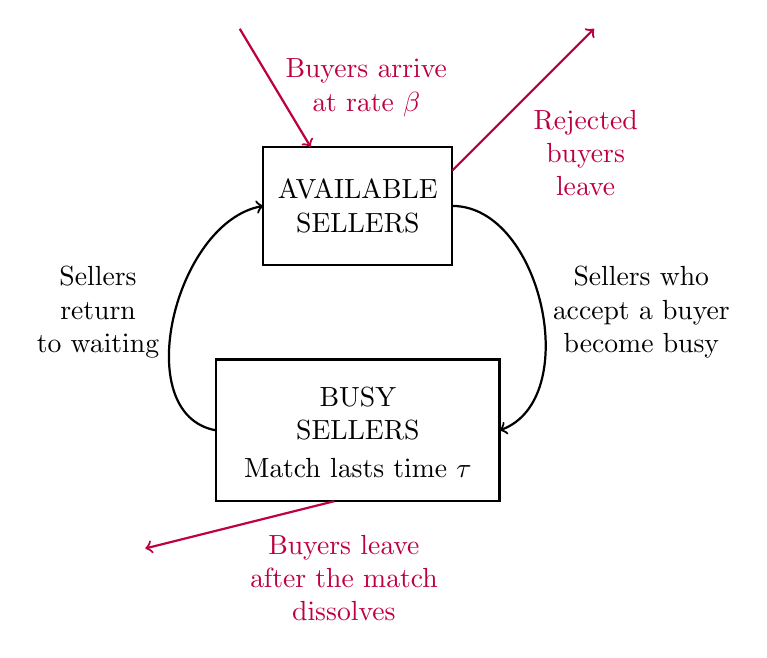
\begin{tikzpicture}[xscale=.6,yscale=.6,xshift=1,yshift=1] 


%	\draw[step=1cm,gray,very thin] (0,0) grid (10,8);

	\draw[thick] (-.5,0) rectangle (5.5,3);
	\node at (2.5,1.5) [align=center] {BUSY\\SELLERS\\};


	\draw[thick] (.5,5) rectangle (4.5,7.5);
	\node at (2.5,6.25) [align=center]  {AVAILABLE\\SELLERS};


	
	\pause


	\draw[thick,->,purple] (0,10) --node[align=center,right] {Buyers arrive\\at rate $\beta$} (1.5,7.5);

	\pause
	\node at (8.5,4) [align=center] {Sellers who\\accept a buyer\\become busy};
	\draw[thick,->,purple] (4.5,7) --node[align=center,below right]{Rejected\\buyers\\leave}++(3,3);
	\draw[thick,->] (4.5,6.25) to [out=0,in=20] (5.5,1.5);

	\pause
	\node at (-3,4) [align=center] {Sellers\\return\\to waiting};
	\draw[thick,->,purple] (2,0) --node[align=center,below right]{Buyers leave\\after the match \\dissolves}++(-4,-1);
	\draw[thick,->] (-.5,1.5) to [out=170,in=-170] (.5,6.25);
	\node at (2.5,.7) [align=center]{Match lasts time $\tau$};



        
\end{tikzpicture}